\section{A otimização combinatória e as colônias de formigas}
\label{chapter:aco}

\subsection{Introdução}

No início da década de 1990, a otimização combinatória com colônias de formigas
(ACO, \textit{Ant Colony
Optimization}) \cite{dorigo1992optimization, dorigo1991positive, dorigo1996ant} surgiu como uma
nova técnica bioinspirada voltada para a solução de problemas difíceis
de otimização combinatória. ACO é uma metaheurística \cite{glover2003handbook},
ou seja, um algoritmo aproximado usado para obter soluções suficientemente
boas para problemas difíceis de otimização combinatória em tempo computacional
razoável. A fonte de inspiração para a metaheurística ACO foi o comportamento
forrageiro das formigas reais. Quando estão procurando por comida, as formigas
inicialmente exploram a área próxima ao seu formigueiro de forma aleatória.
Assim que uma formiga descobre alguma fonte de comida, ela avalia a fonte e
transporta um pouco de volta para o formigueiro. Nesse caminho de volta, a
formiga deposita uma trilha de feromônios --
substâncias químicas capazes de despertar reações fisiológicas ou
comportamentais em outros membros de uma mesma espécie que estejam num
determinado raio de espaço físico ocupado pelo excretor
\cite{karlson1959pheromones}. A quantidade de feromônio depositada, que pode
depender da quantidade e qualidade da comida, vai guiar outras formigas até a
fonte de comida. A comunicação indireta entre as formigas por meio das trilhas
de feromônios as torna capazes de encontrar o caminho mais curto entre o
formigueiro e a fonte de comida \cite{deneubourg1990self}. Essa característica
das colônias de formigas reais é explorada em colônias de formigas
artificiais, sendo a base da ACO. A Figura \ref{fig:formigueiro} mostra essa
característica. Em (i), vê-se uma formiga retornando da fonte de comida para o
formigueiro, deixando um rastro de feromônio pelo caminho percorrido. Em (ii)
são retratadas várias formigas indo do formigueiro à fonte de comida por
caminhos diferentes, e marcando esses caminhos com feromônio. As formigas que
escolhem o menor caminho retornam primeiro, e o nível de feromônio nesta
trilha vai se tornando mais acentuado com o tempo, aumentando a probabilidade
de futuras formigas escolherem esse caminho. (iii) mostra essa convergência,
onde, após algum tempo, a maior parte das formigas passa a utilizar o caminho
mais curto.

\begin{figure}
\centering
 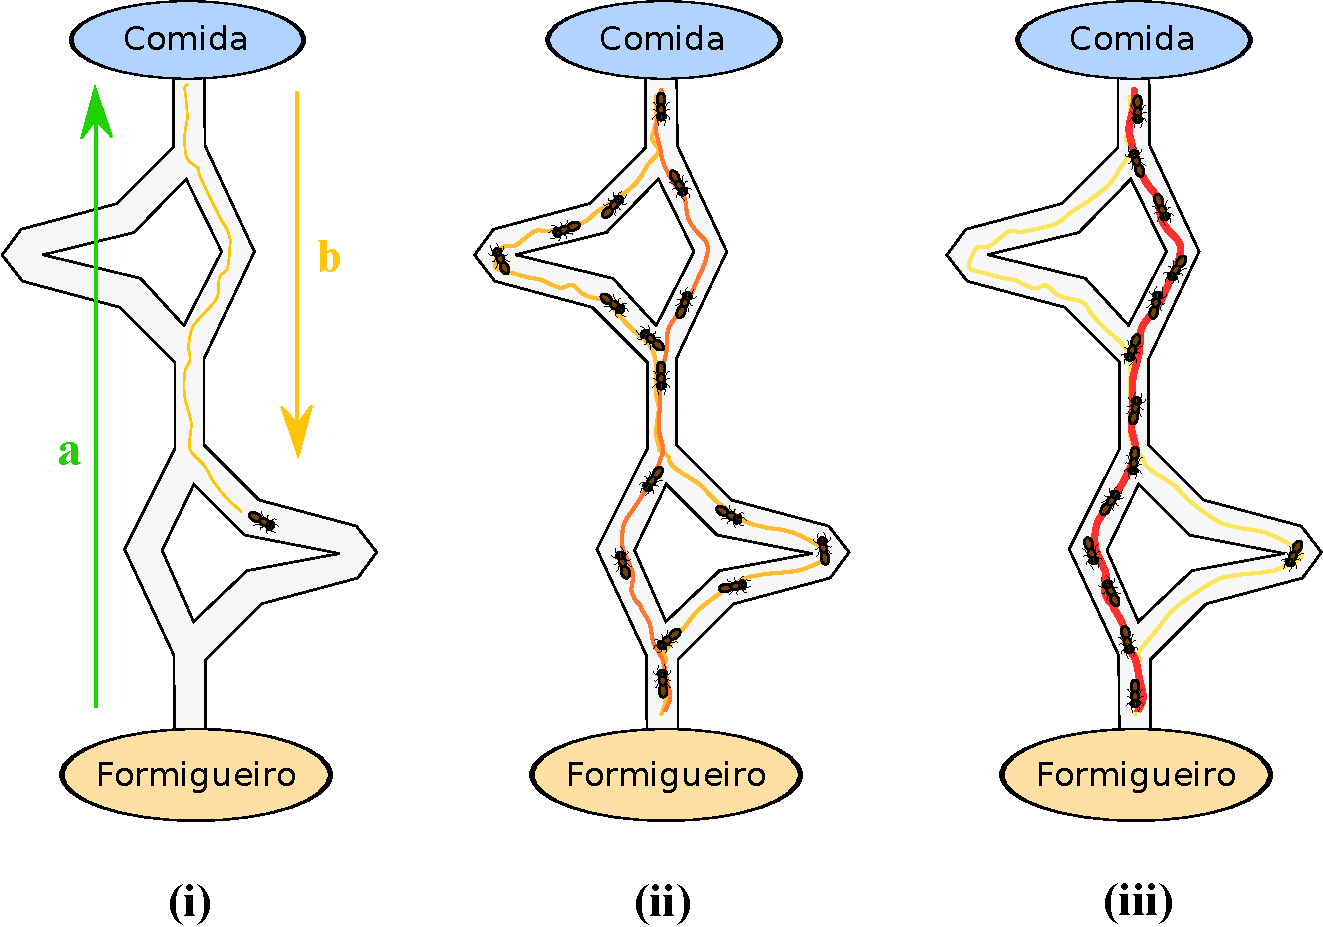
\includegraphics[scale=0.5]{fig/formigueiro-crop.pdf}
\caption{Colônia de formigas}
\label{fig:formigueiro}
\end{figure}


\subsection{Otimização combinatória}
A otimização combinatória é um ramo da matemática aplicada e da ciência da
computação que lida com a solução de problemas que podem ser catacterizados
como possuindo uma estrutura discreta ou combinatória. Estes problemas são
modelados com uma função objetivo e envolvem achar valores para variáveis
discretas tal que seja encontrada uma solução ótima para essa função objetivo.
Muitos dos problemas de otimização de importância teórica e prática são de
natureza combinatória, como por exemplo encontrar o melhor esquema de roteamento
de pacotes em uma rede, a melhor maneira de se alocar professores e disciplinas ou a
melhor maneira de se visitar um determinado conjunto de lugares diferentes. 

Um problema de otimizaçao combinatória ou é de maximização ou de minimização, e
tem associado um conjunto de instâncias do problema. Aqui, \textit{problema} se
refere à pergunta a ser respondida, geralmente contendo vários parâmetros ou
variáveis com valores não especificados. Uma \textit{instância} se refere a um
problema com os valores especificados para cada parâmetro.

Formalmente, um problema de otimização combinatória $\Pi$ é uma tripla
$(\mathcal{S}, f, \Omega)$, onde $\mathcal{S}$ é o conjunto de soluções, $f$ é
a função objetivo que atribui um valor $f(s)$ a cada solução $s \in
\mathcal{S}$, e $\Omega$ é um conjunto de restrições. As soluções pertencentes
ao conjunto $\tilde{\mathcal{S}} \subseteq \mathcal{S}$ que satisfazem às
restrições $\Omega$ são chamadas soluções viáveis. A idéia é encontrar uma
solução $s^{*}$, viável, que seja um ótimo global, ou seja, ótima dentre
todas as soluções viáveis. Num problema de maximização, $s^{*}$ seria a solução
viável com o maior valor da função objetivo $f$, ao passo que, num problema de
minimização, $s^{*}$ seria a solução viável com o menor valor de $f$.

\subsection{O que é uma metaheurística?}
Uma metaheurística é um conjunto de conceitos algorítmicos que podem ser usados
para definir métodos heurísticos aplicáveis a uma diversidade de problemas
\cite{975277}. Uma metaheurística seria então um \textit{framework} algorítmico
que pode ser aplicado a diferentes problemas de otimização com relativamente
poucas modificações para torná-lo adaptado ao problema específico.

Como exemplos de metaheurísticas podemos citar algoritmos evolucionários, como
o \textit{Non-dominated Sorting Genetic Algorithm} (NSGA)
\cite{Srinivas94multiobjectiveoptimization}, o NSGA-II \cite{deb2002fast}, o
\textit{Strength Pareto Evolutionary Algorithm} (SPEA)
\cite{zitzler1998evolutionary} e o SPEA-II \cite{zitzler2001spea2}; algoritmos
probabilísticos, como o \textit{Bayesian Optimization Algorithm} (BOA)
\cite{Cantu-Paz98linkageproblem}, o \textit{Expectation-maximization
algorithm} (EM) \cite{moon1996expectation} e o \textit{Compact Genetic
Algorithm} \cite{harik1998compact}; algoritmos estocásticos, como o
\textit{Tabu Search} \cite{glover1990tabu}; e também algoritmos baseados em
inteligência coletiva, como algoritmos baseados em abelhas
\cite{teodorovic2005bee}, cupins \cite{roth2003termite}, e finalmente, em
formigas, \textit{Ant Colony Optimization} (ACO) \cite{dorigo1992optimization},
que será detalhado na próxima seção.

\subsection{Otimização combinatória com colônias de formigas - a metaheurística}
\label{sec:atsp}
Algoritmos ACO são procedimentos de busca
estocástica centrados em um modelo de feromônio, que é usado para tomar
amostras -- probabilisticamente -- dentro de um espaço de busca.

Como exemplo, vamos formular o problema do caixeiro viajante assimétrico
(ATSP,
\textit{Assymetric Traveling Salesman Problem}) a seguir. O problema em si
consiste em um grafo dirigido, completamente conectado $G(V, A)$, com um peso
positivo $d_{ij}$ associado a cada arco $a_{ij} \in A$. Os nós do grafo
representam cidades, e os pesos dos arcos, as distâncias entre elas. O objetivo
é encontrar, dentre todos os ciclos Hamiltonianos \footnote{Um ciclo ou caminho
hamiltoniano é um caminho que permite passar por todos os vértices de um grafo
G não repetindo nenhum, ou seja, passar por cada nó uma e apenas uma vez.} de
$G$, o de custo mínimo, o custo sendo a soma dos pesos de todos os seus arcos.
Este problema de otimização combinatória pode ser modelado da seguinte forma:
cada cidade $i \in V$ é modelada por uma variável de decisão $X_{i}$ cujo
domínio consiste de um valor $v_{i}^{j}$ para cada arco $a_{ij}$. A instância
de uma variável $X_{i} = v_{i}^{j}$ significa que o arco $a_{ij}$ é parte da
solução considerada. O conjunto de restrições é definido tal que somente
soluções candidatas que correspondam aos ciclos Hamiltonianos de $G$ são
soluções válidas. O conjunto de componentes de soluções $\mathcal{C}$ consiste
de um componente de solução $c_{i}^{j}$ para cada combinação de variável
$X_{i}$ e valor de domínio $v_{i}^{j}$, e o modelo de feromônio $\mathcal{T}$
consiste de uma trilha de feromônio $\mathcal{T}_{i}^{j}$, com um valor
$\tau_{i}^{j}$ associado a cada componente de solução $c_{i}^{j}$. 

\subsubsection{Um framework ACO simples}
O algoritmo \ref{algo:aco} mostra o \textit{framework} de um algoritmo ACO
básico, que funciona como segue: A cada iteração, $n_{a}$ formigas
probabilisticamente constróem soluções para o problema de otimização
combinatória considerado, explorando um dado modelo de feromônio, e
, opcionalmente, um procedimento de busca local é aplicado às soluções
construídas. Finalmente, antes da próxima iteração, algumas das soluções são
utilizadas na execução da atualização de feromônio. Este \textit{framework},
que foi descrito em \cite{dorigo2005ant}, será explicado com mais detalhes a
seguir.

\begin{algorithm}[h]
\label{algo:aco}
\caption{\textit{Framework} de um algoritmo ACO básico}
\Entrada{Uma instância $\mathcal{P}$ de um problema de otimização combinatória}
Inicializa os Feromônios($\mathcal{T}$)\;
$s_{melhor} \gets NULL$\;
\Enqto{condições de saída não forem satisfeitas}{
$\mathcal{C}_{iter} \gets \emptyset$\;
\Para{$i = 1, \ldots, n_{a}$} {
$s \gets$ Constrói Solução($\mathcal{T}$)\;
\Se{$s$ é uma solução válida} {
$s \gets$ Busca Local($s$) /* opcional */\;
\Se{($f(s) < f(s_{melhor})$) ou ($s_{melhor} = NULL$)} {
$s_{melhor} \gets s$\;
}
$\mathcal{C}_{iter} \gets \mathcal{C}_{iter} \cup \{s\}$
}
}
Atualiza Feromônio($\mathcal{T}, \mathcal{C}_{iter}, s_{melhor}$)\;
}
\Saida{A melhor solução até o momento, $s_{melhor}$}
\end{algorithm}

Inicializa os Feromônios($\mathcal{T}$). No início do algoritmo, os valores de
feromônio são todos inicializados com uma constante $c > 0$. 

Constrói Solução($\mathcal{T}$). O componente fundamental de qualquer algoritmo
ACO é uma heurística construtiva para a contrução probabilística das soluções.
Uma heurística construtiva monta soluções como sequências de elementos do
conjunto finito de componentes de solução $\mathcal{C}$. A construção de uma
solução começa com um conjunto vazio de soluções parciais $s_{parcial} =
\langle \rangle$, e a cada passo da construção, o conjunto de soluções parciais
é estendido adicionando-se um componente de solução viável do conjunto
$\mathcal{R}(s_{parcial}) \subseteq \mathcal{C} \setminus \{s_{parcial}\}$.
Este conjunto é determinado a cada passo do mecanismo de construção da solução
de modo que as restrições do problema são satisfeitas. O processo de construção
de soluções pode ser visualizado como o caminhamento no chamado grafo de
construção $G_{c} = (\mathcal{C}, \mathcal{L})$, que é um grafo completamente
conectado, cujos vértices são os componentes de solução em $\mathcal{C}$ e
cujas arestas são os elementos de $\mathcal{L}$. Os caminhamentos permitidos em
$G_{c}$ são definidos implicitamente pelo mecanismo de construção de solução
que define o conjunto $\mathcal{R}(s_{parcial})$ com respeito à solução parcial
$s_{parcial}$. A escolha de um componente de solução $c_{i}^{j} \in
\mathcal{R}(s_{parcial})$ é, em cada passo de construção, feito
probabilisticamente com respeito ao modelo de feromônio adotado. A
probabilidade para a escolha $c_{i}^{j}$ é proporcional a
$[\tau_{i}^{j}]^{\alpha} \cdot [n(c_{i}^{j})]^{\beta}$, onde $n$ é uma função
que atribui a cada componente de solução válida um valor heurístico que é
também conhecido como \textit{informação heurística}. Os valores dos parâmetros
$\alpha$ e $\beta$, $\alpha > 0$ e $\beta > 0$, determinam a importância
relativa dos valores de feromônio e da informação heurística. A informação
heurística é opcional, mas geralmente necessária quando se pretende alcançar
uma alta performance do algoritmo. Na maioria dos algoritmos ACO, as
probabilidades de se escolher o próximo componente de solução -- também chamada
de probabilidade de transição -- são definidas como segue:
\begin{equation}
\label{eq:acoprob}
P(c_{i}^{j} \mid s_{parcial}) = \frac{[\tau_{i}^{j}]^{\alpha} \cdot
[n(c_{i}^{j})]^{\beta}}{\sum_{c_{k}^{l} \in \mathcal{R}(s_{parcial})}
[\tau_{i}^{j}]^{\alpha} \cdot [n(c_{i}^{j})]^{\beta}}, \forall c_{i}^{j} \in
\mathcal{R}(s_{parcial})
\end{equation}

Na prática, há diversas formas de se escolher as probabilidades de transição,
mas a ilustrada em (\ref{eq:acoprob}) é tida como tradicional por ter sido
utilizada nos primeiros algoritmos ACO propostos, \cite{dorigo1991positive} e
\cite{dorigo1996ant}.

Voltando ao ATSP, definido em \ref{sec:atsp}, vamos denotar por $\mathcal{I}$ o
conjunto de índices da variável de decisão atual e das variáveis de decisão que
já têm um valor atribuído. A construção da solução começa com um conjunto de
soluções parciais vazio, $s_{parcial} = \langle \rangle$, com $i_{c} \in \{1,
\ldots, |V|\}$ escolhido aleatoriamente com $\mathcal{I} = \{i_{c}\}$. O índice
da primeira variável de decisão é armazenado na variável $i_{primeira}$. Então,
em cada dos $|V|-1$ passos de construção, um componente de solução $c_{i}^{j}
\in \mathcal{R}(s_{parcial})$ é adicionado à solução parcial, onde
$\mathcal{R}(s_{parcial}) = \{c_{i_{c}}^{k}\}\ |\ k \in \{1, \ldots, |V|\}
\setminus \mathcal{I}\}$. Isto significa que em cada passo de construção, um
valor de domínio é escolhido para a variável de decisão com índice $i_{c}$. Uma
vez que o componente de solução $c_{i_{c}}^{j}$ seja adicionado a
$s_{parcial}$, $i_{c}$ recebe o valor $j$. As probabilidades de transição
usadas em cada um dos primeiros $|V|-1$ passos de construção são as definidas
pela equação (\ref{eq:acoprob}). No ATSP, a informação heurística pode ser
definida como $n(c_{i}^{j}) = d_{ij}^{-1}$ (esta escolha dá preferência aos
menores caminhos). O último passo de construção consiste em adicionar o
componente de solução $c_{i_{c}}^{i_{primeira}}$ à solução parcial
$s_{parcial}$, que corresponde ao fechamento do ciclo Hamiltoniano.

Busca Local($s$). Um procedimento de busca local pode ser aplicado para
melhorar as soluções construídas pelas formigas. O uso de tal procedimento é
opcional, mas experimentos mostraram que, quando disponível, seu uso melhora o
desempenho geral do algoritmo \cite{dorigo2005ant}.

Atualiza Feromônio($\mathcal{T}, \mathcal{C}_{iter}, s_{melhor}$). A idéia por
trás da regra de atualização de feromônio é aumentar o nível de feromônio das
melhores soluções. Segundo \cite{dorigo2005ant}, a maioria dos algoritmos ACO
utiliza uma variação da regra de atualização (\ref{eq:acoupdate}).
\begin{equation}
\label{eq:acoupdate}
\tau_{i}^{j} \gets (1 - \rho) \cdot \tau_{i}^{j} +
\frac{\rho}{\mathcal{C}_{atualizacao}} \cdot \sum_{\{s \in
\mathcal{C}_{atualizacao} | c_{i}^{j} \in s\}} F(s),
\end{equation}

para $i = 1, \ldots n$, e $j = 1, \ldots |D_{i}|$. Instâncias desta regra de
atualização são obtidas com diferentes especificações de
$\mathcal{C}_{atualizacao}$, que é um subconjunto de $\mathcal{C}_{iter} \cup
\{s_{melhor}\}$, onde $\mathcal{C}_{iter}$ é o conjunto de soluções que foram
construídas na iteração atual, e $s_{melhor}$, a melhor solução até o momento.
O parâmetro $\rho \in (0, 1]$ é conhecido como \textit{taxa de evaporação}, e
tem a função de decrementar todos os valores de feromônio de modo uniforme. De
um ponto de vista prático, a evaporação é necessária para evitar uma
convergência muito rápida do algoritmo em direção a uma região subótima, ou
seja, é uma maneira de se escapar de um ótimo local, favorecendo a exploração
de novas áreas no espaço de busca. $F: \mathcal{C} \mapsto \mathcal{R}^{+}$ é
uma função tal que $f(s) < f(s') \Rightarrow +\infty > F(s) \geq F(s'), \forall
s \neq s' \in \mathcal{C}$, onde $\mathcal{C}$ é o conjunto de todas as
sequências de componentes de solução que podem ser construídas pelo algoritmo
ACO e que correspondem a soluções viáveis. $F(\cdot)$ é conhecida como
\textit{função qualidade}. Note que o fator $\mathcal{C}_{atualizacao}^{-1}$
não é usado, normalmente, mas foi introduzido meramente para se estudar os
valores esperados de atualização dos níveis de feromônio. Na maioria dos
algoritmos, este fator é constante, portanto não muda o comportamento
qualitativo do algoritmo em questão \cite{dorigo2005ant}.

% 

% 
% 
% 
% \section{Roteamento baseado em inteligência coletiva}
% 
% 
% 
% \cite{joerg2004ants} \cite{rosati2008ant} \cite{bernet2006simulation}
